\section{Experimentación}
Llegado el momento de la experimentación, se tenía una base de datos de imágenes divididas entre
resoluciones de 112 x 92 píxeles y de 28 x 23 píxeles y se decidió divivir los tests de igual forma.

A los tests hechos sobre las imágenes de 28 x 23 se los subdividió en dos, tests con el método 0 y
tests con el método 1. Esto hace referencia al método empleado para buscar los autovectores y
autovalores de la matriz de covarianzas. El método 0 consistía en hacerlo sobre la matriz $A^t A$
mientras que el método 1 consistía en hacerlo sobre la matriz $A A^t$.

Por el lado de las imágenes de 112 x 92 pixeles se volvió inviable el método 0, dado que la
dimension de la matriz terminaría siendo de $(112*92)^2 > 106$ millones de celdas mientras que la
matriz del método 1 tendría \textbf{cómo máximo} $(41*10)^2 = 168 100$ celdas si usamos a todas las
imágenes.

En cada una de las subdivisiones se testeó lo siguiente al ir aumentando el K, o la cantidad de
autovectores:
\begin{compactitem}
  \item \textbf{Mediciones de TK}: mide el tiempo de obtener la matriz de autovectores. Es decir:
  \begin{compactenum}
    \item Restarle el $\mu$ y dividir por $\sqrt{n-1}$ a la matriz
    \item Tiempo de calcular los K autovectores
    \item Tiempo de multiplicar por izquierda al autovector de $A A^t$ por $A^t$ para obtener el
    autovector con el mismo autovalor pero de $A^t A$.
  \end{compactenum}
  Se varía entre 1, 5 y 10 muestras para 11, 21 y 41 personas.
  \item \textbf{Mediciones de Ttodos}: el tiempo de identificar a todos los sujetos usando el método
  de identificación del vecino más cercano. Incluye el tiempo de restarle el $\mu$ y dividir por
  $\sqrt{n-1}$ a la matriz. Se varía entre 1, 5 y 10 muestras para 11, 21 y 41 personas.
  \item \textbf{Mediciones de Tcentro}: el tiempo de identificar a todos los sujetos usando el método
  de identificación de los centros de masa. Incluye el tiempo de restarle el $\mu$ y dividir por
  $\sqrt{n-1}$ a la matriz. Se varía entre 1, 5 y 10 muestras para 11, 21 y 41 personas.
  \item \textbf{Mediciones de HitsTodos}: el coeficiente entre los \textit{hits} al identificar un
  sujeto y la cantidad de estos usando el método del vecino más cercano. Se varía entre 1, 3, 5, 7,
  9 y 10 muestras para 11, 21 y 41 personas.
  \item \textbf{Mediciones de HitsCentro} el coeficiente entre los \textit{hits} al identificar un
  sujeto y la cantidad de estos usando el método de los centros de masa. Se varía entre 1, 3, 5, 7,
  9 y 10 muestras para 11, 21 y 41 personas.
\end{compactitem}

Para los tests, eligiremos mostrar cómo se irán comportando estas mediciones acorde aumente el K.
Además, para una cantidad fija de personas, cuando decimos, por ejemplo, \textit{se varía
  entre 1, 5 y 10 muestras}, nos referimos a que medimos 3 instancias distintas. La primera, con una
muestra, se refiera a que de la base de datos se elige aleatoriamente una muestra por cada persona
para calcular la matriz inicial y, por ende, la matriz de autovectores. Además, se elige para
identificar por cada persona una muestra que no haya sido usada para generar la matriz inicial. En
el caso de 5 muestras, se genera la matriz usando 5 muestras por persona y de nuevo por cada una de
las personas tenidas en cuenta, se trata de identificar una de sus muestras que no haya sido usada
para calcular la matriz inicial.

El caso \textbf{distinto} sería el caso de 10 muestras. Aquí, dado que se usan todas las muestras
disponibles para cada una de las personas para generar la matriz inicial, no quedan muestras libres
para identificar por cada persona. En ese caso se elige una muestra random y se testea qué tan
buenos son los métodos de reconocimiento cuando se trata de identificar a alguien perteneciente a la
base de datos.


% Con muestras nos referimos a cantidad de muestras por persona usadas para calcular la matriz de
% autovectores. En el caso de las personas a identificar, se elige una muestra random que no haya sido
% usada en el cálculo de los autovectores.

Sobre estos tests esperamos encontrar que:
\begin{compactitem}
  \item Los tiempos son crecientes acorde al incremento de los autovectores buscados dado que
  mientras más grande sea la matriz de autovectores, más tiempo se tardará en encontrarla y, en el
  caso del método 1, se deberá multiplicar por izquierda a cada autovector para trasladarlo a un
  autovector de la matriz de $A^t A$.
  \item Los tiempos del método 1 deben ser mucho menores a los tiempos del método 0.
  \item El coeficiente de HitsTodos debe ser siempre 1 para los casos en los que se usen 10 muestras
  dado que toda muestra a identificar ha sido usada para generar la matriz de autovectores y,
  además, este método de identificación compara con todos los puntos, y entre ellos va a estar él
  mismo, que terminaría siendo el más cercano.
  \item Los coeficientes de HitsTodos y HitsCentro deben aumentar acorde aumenten la cantidad de
  muestras y la cantidad de autovectores.
\end{compactitem}


\section{Resultados}
\subsection{Experimentacion con Imagenes Reducidas}
\subsubsection{Metodo 0: Utilizando $A^tA$}

\textbf{Mediciones de TK}
\begin{figure}[H]
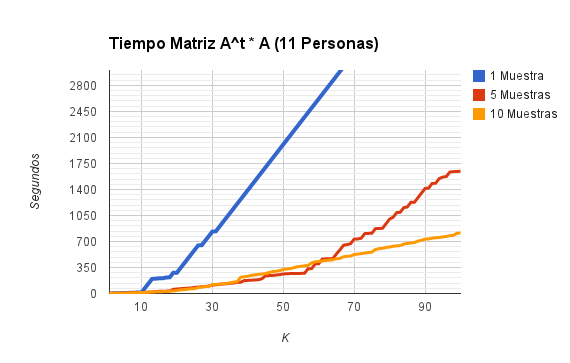
\includegraphics[width=1\textwidth]{img/image1.png}
     \caption{Tiempos Matrix $A^tA$ con 11 personas variando K}
     \label{fig:figura1}
\end{figure}

\begin{figure}[H]
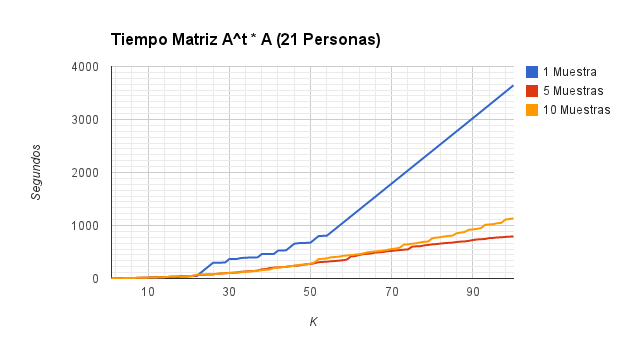
\includegraphics[width=1\textwidth]{img/image2.png}
     \caption{Tiempos Matrix $A^tA$ con 21 personas variando K}
     \label{fig:figura1}
\end{figure}

\begin{figure}[H]
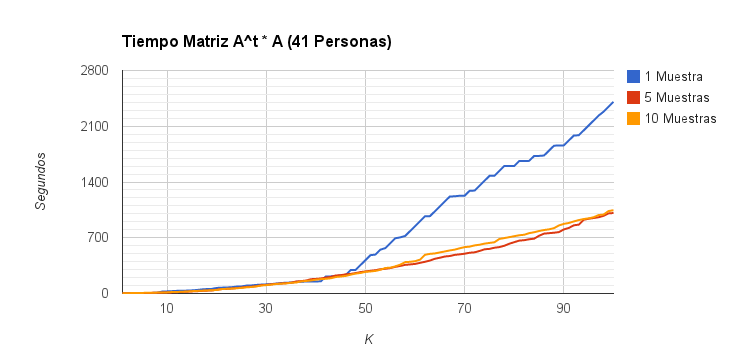
\includegraphics[width=1\textwidth]{img/image3.png}
     \caption{Tiempos Matrix $A^tA$ con 41 personas variando K}
     \label{fig:figura1}
\end{figure}


\textbf{Mediciones de Ttodos }

\begin{figure}[H]
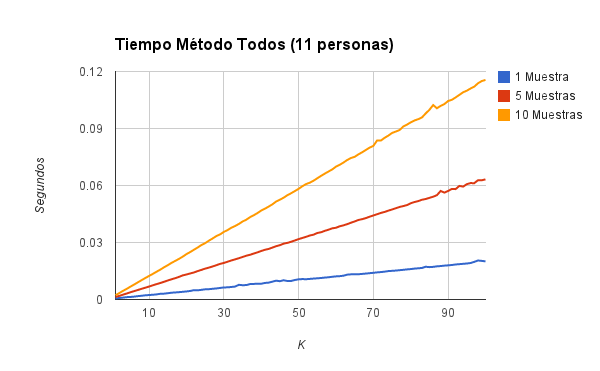
\includegraphics[width=1\textwidth]{img/image4.png}
     \caption{Tiempos Todos \textcolor{red}{??} Matrix $A^tA$ con 11 personas variando K}
     \label{fig:figura1}
\end{figure}

\begin{figure}[H]
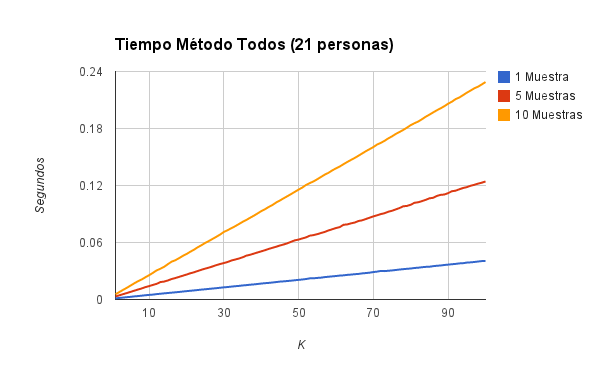
\includegraphics[width=1\textwidth]{img/image5.png}
     \caption{Tiempos Todos \textcolor{red}{??} Matrix $A^tA$ con 21 personas variando K}
     \label{fig:figura1}
\end{figure}

\begin{figure}[H]
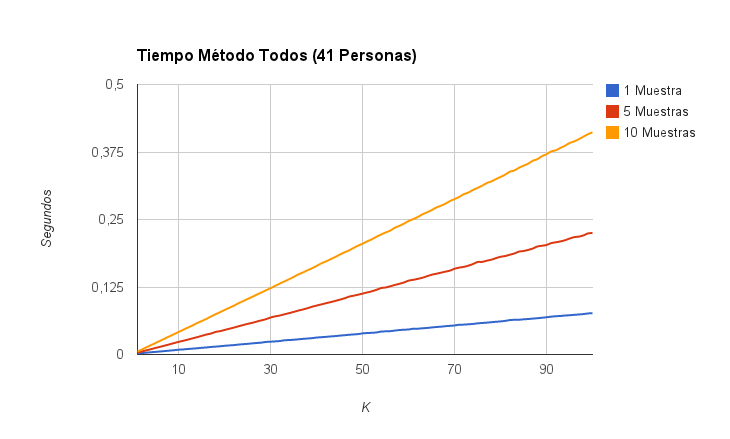
\includegraphics[width=1\textwidth]{img/image6.png}
     \caption{Tiempos Todos \textcolor{red}{??} Matrix $A^tA$ con 41 personas variando K}
     \label{fig:figura1}
\end{figure}


\textbf{Mediciones de Tcentro }

\begin{figure}[H]
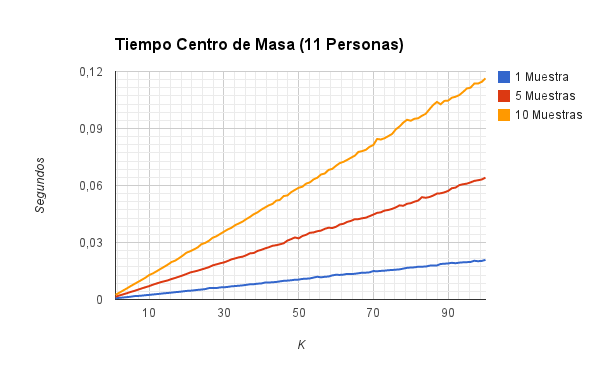
\includegraphics[width=1\textwidth]{img/image7.png}
     \caption{Tiempos Centro \textcolor{red}{??} Matrix $A^tA$ con 11 personas variando K}
     \label{fig:figura1}
\end{figure}

\begin{figure}[H]
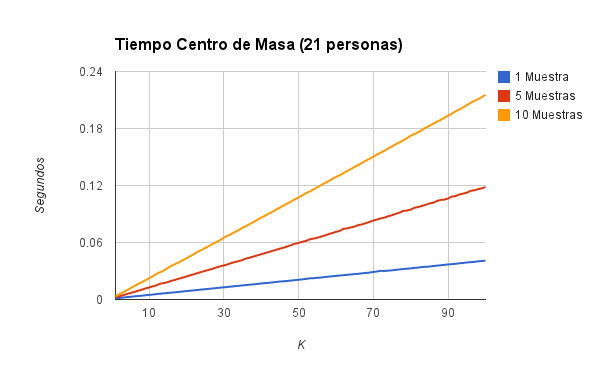
\includegraphics[width=1\textwidth]{img/image8.png}
     \caption{Tiempos Centro \textcolor{red}{??} Matrix $A^tA$ con 21 personas variando K}
     \label{fig:figura1}
\end{figure}

\begin{figure}[H]
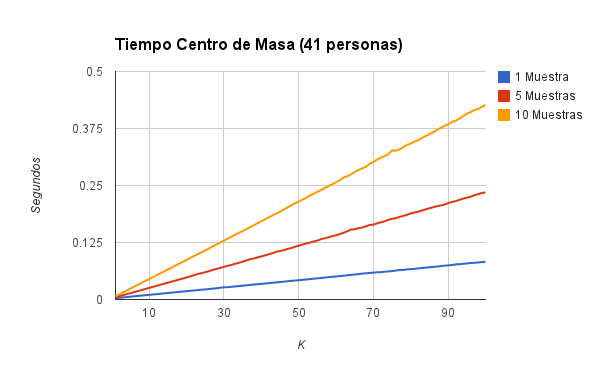
\includegraphics[width=1\textwidth]{img/image9.png}
     \caption{Tiempos Centro \textcolor{red}{??} Matrix $A^tA$ con 41 personas variando K}
     \label{fig:figura1}
\end{figure}



\textbf{Mediciones de HitsTodos }

\begin{figure}[H]
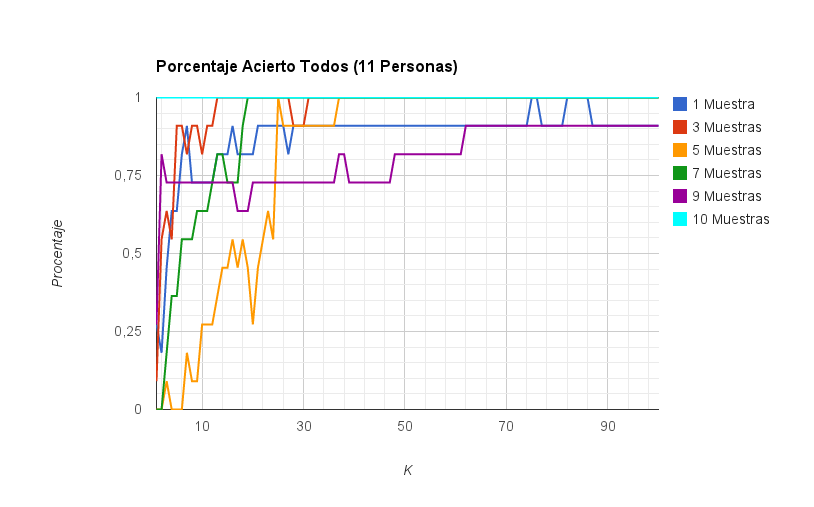
\includegraphics[width=1\textwidth]{img/image10.png}
     \caption{Tiempos HitTodos \textcolor{red}{??} Matrix $A^tA$ con 11 personas variando K}
     \label{fig:figura1}
\end{figure}

\begin{figure}[H]
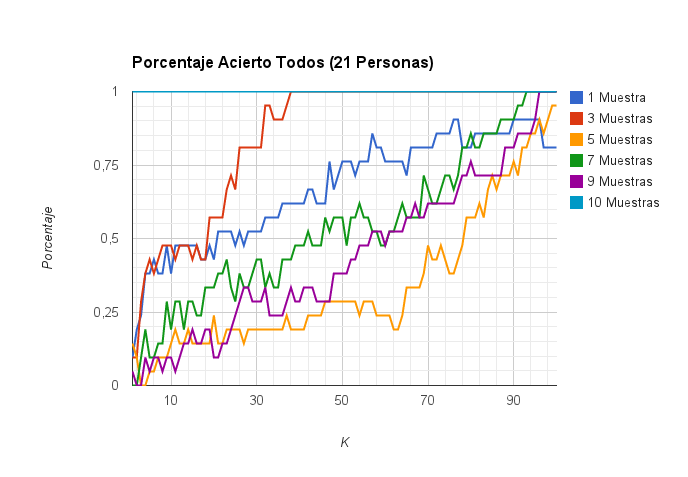
\includegraphics[width=1\textwidth]{img/image11.png}
     \caption{Tiempos HitTodos \textcolor{red}{??} Matrix $A^tA$ con 21 personas variando K}
     \label{fig:figura1}
\end{figure}

\begin{figure}[H]
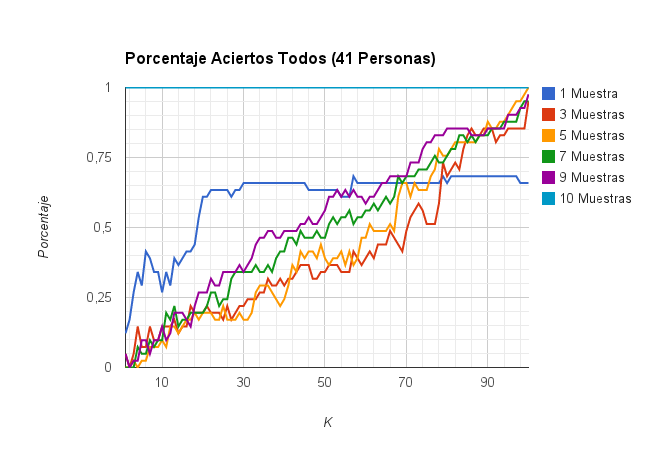
\includegraphics[width=1\textwidth]{img/image12.png}
     \caption{Tiempos HitTodos \textcolor{red}{??} Matrix $A^tA$ con 41 personas variando K}
     \label{fig:figura1}
\end{figure}





\textbf{Mediciones de HitsCentro }

\begin{figure}[H]
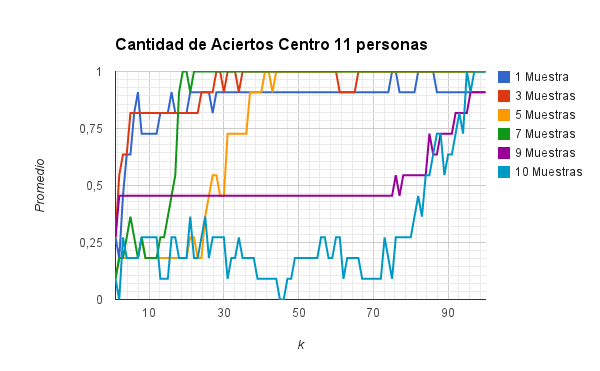
\includegraphics[width=1\textwidth]{img/image13.png}
     \caption{Tiempos HitsCentro \textcolor{red}{??} Matrix $A^tA$ con 11 personas variando K}
     \label{fig:figura1}
\end{figure}

\begin{figure}[H]
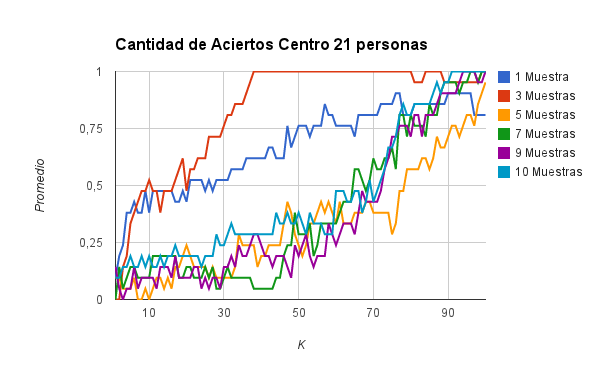
\includegraphics[width=1\textwidth]{img/image14.png}
     \caption{Tiempos HitsCentro \textcolor{red}{??} Matrix $A^tA$ con 21 personas variando K}
     \label{fig:figura1}
\end{figure}

\begin{figure}[H]
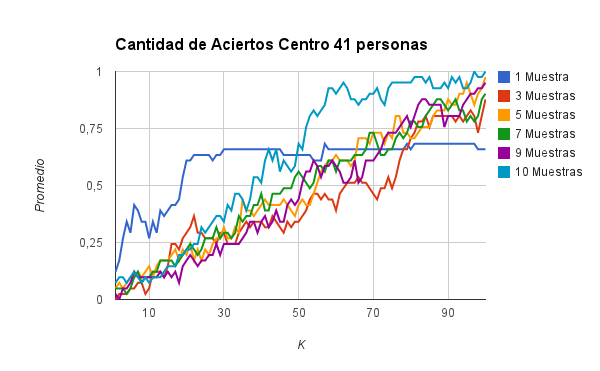
\includegraphics[width=1\textwidth]{img/image15.png}
     \caption{Tiempos HitsCentro \textcolor{red}{??} Matrix $A^tA$ con 41 personas variando K}
     \label{fig:figura1}
\end{figure}

\textbf{Conclusiones:}

\textcolor{red}{EXPLICAR}


\subsubsection{Metodo 1: Utilizando $AA^t$}

\textbf{Mediciones de TK }

\begin{figure}[H]
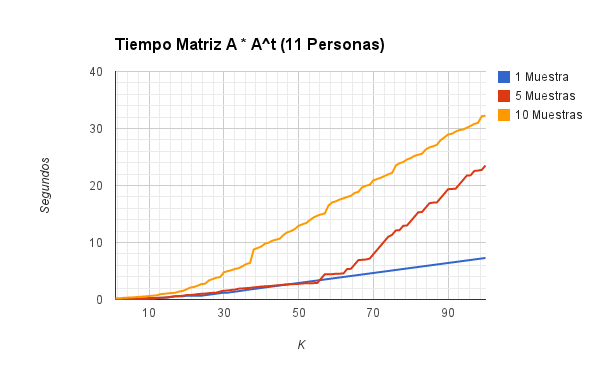
\includegraphics[width=1\textwidth]{img/imagea.png}
     \caption{Tiempos Matrix $A^tA$ con 11 personas variando K}
     \label{fig:figura1}
\end{figure}

\begin{figure}[H]
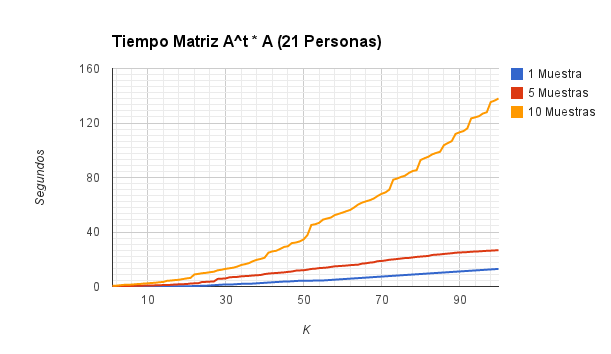
\includegraphics[width=1\textwidth]{img/imageb.png}
     \caption{Tiempos Matrix $A^tA$ con 21 personas variando K}
     \label{fig:figura1}
\end{figure}

\begin{figure}[H]
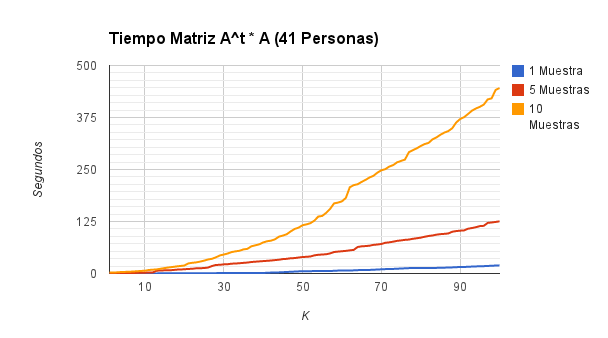
\includegraphics[width=1\textwidth]{img/imagec.png}
     \caption{Tiempos Matrix $A^tA$ con 41 personas variando K}
     \label{fig:figura1}
\end{figure}


\textbf{Mediciones de Ttodos }

\begin{figure}[H]
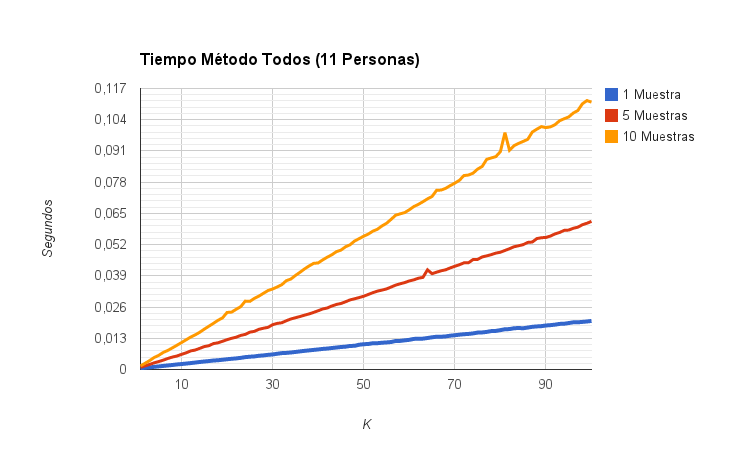
\includegraphics[width=1\textwidth]{img/imaged.png}
     \caption{Tiempos Todos \textcolor{red}{??} Matrix $A^tA$ con 11 personas variando K}
     \label{fig:figura1}
\end{figure}

\begin{figure}[H]
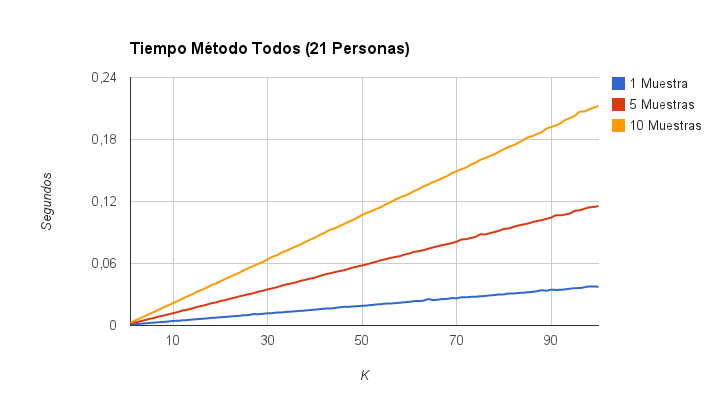
\includegraphics[width=1\textwidth]{img/imagee.png}
     \caption{Tiempos Todos \textcolor{red}{??} Matrix $A^tA$ con 21 personas variando K}
     \label{fig:figura1}
\end{figure}

\begin{figure}[H]
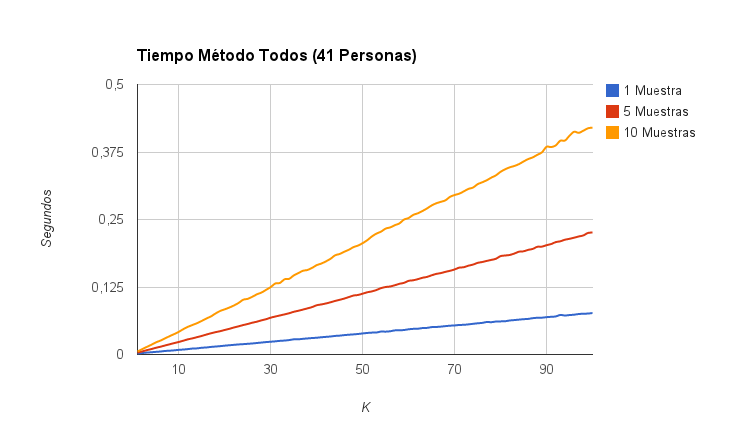
\includegraphics[width=1\textwidth]{img/imagef.png}
     \caption{Tiempos Todos \textcolor{red}{??} Matrix $A^tA$ con 41 personas variando K}
     \label{fig:figura1}
\end{figure}

\textbf{Mediciones de Tcentro }

\begin{figure}[H]
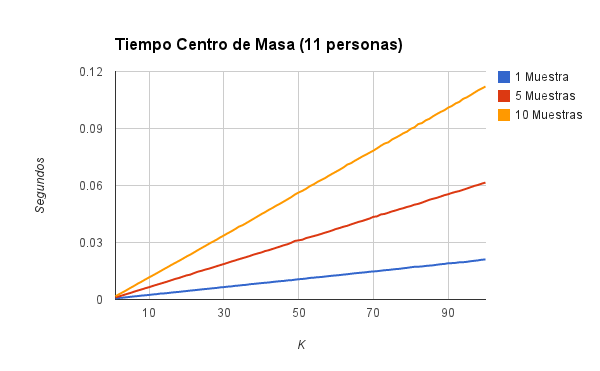
\includegraphics[width=1\textwidth]{img/imageg.png}
     \caption{Tiempos Centro \textcolor{red}{??} Matrix $A^tA$ con 11 personas variando K}
     \label{fig:figura1}
\end{figure}

\begin{figure}[H]
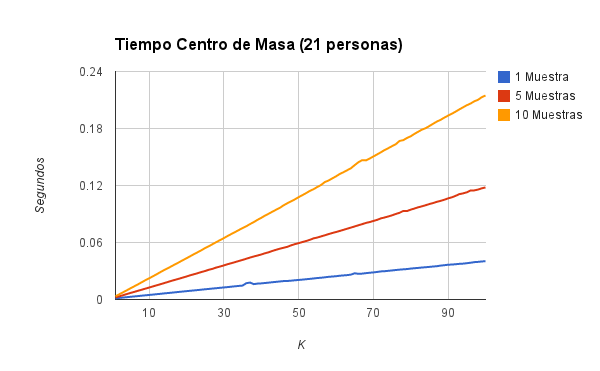
\includegraphics[width=1\textwidth]{img/imageh.png}
     \caption{Tiempos Centro \textcolor{red}{??} Matrix $A^tA$ con 21 personas variando K}
     \label{fig:figura1}
\end{figure}

\begin{figure}[H]
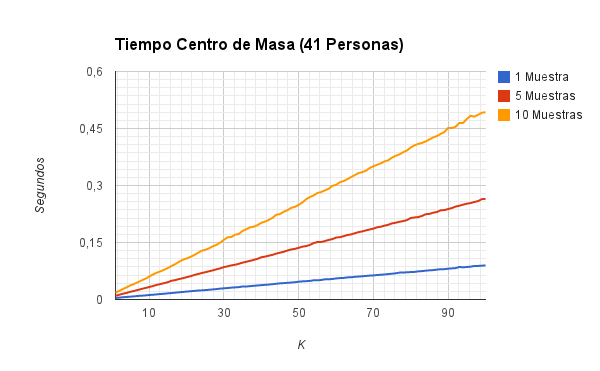
\includegraphics[width=1\textwidth]{img/imagei.png}
     \caption{Tiempos Centro \textcolor{red}{??} Matrix $A^tA$ con 41 personas variando K}
     \label{fig:figura1}
\end{figure}


\textbf{Mediciones de HitsTodos}

\begin{figure}[H]
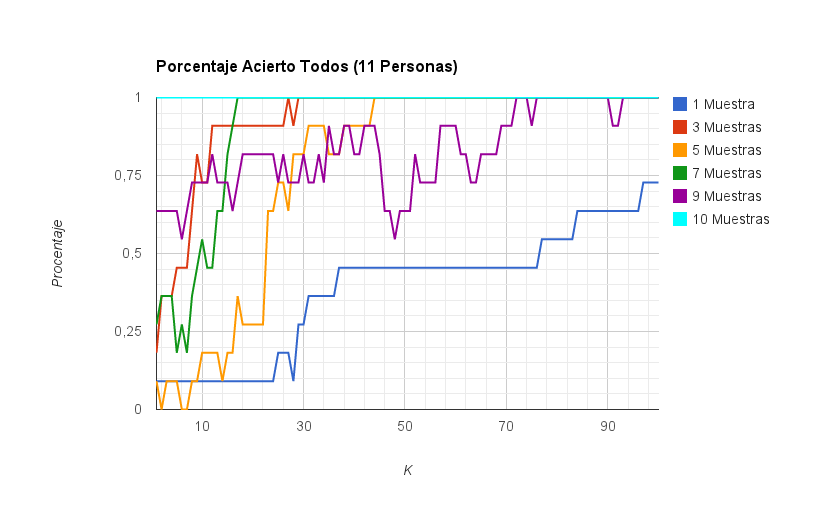
\includegraphics[width=1\textwidth]{img/imagej.png}
     \caption{Tiempos HitTodos \textcolor{red}{??} Matrix $A^tA$ con 11 personas variando K}
     \label{fig:figura1}
\end{figure}

\begin{figure}[H]
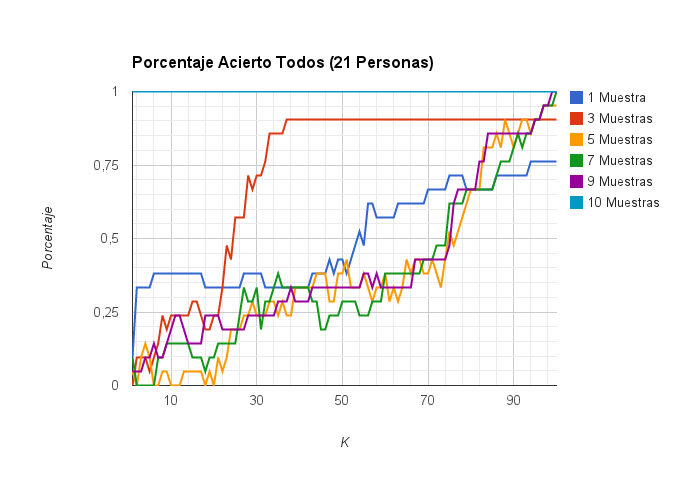
\includegraphics[width=1\textwidth]{img/imagek.png}
     \caption{Tiempos HitTodos \textcolor{red}{??} Matrix $A^tA$ con 21 personas variando K}
     \label{fig:figura1}
\end{figure}

\begin{figure}[H]
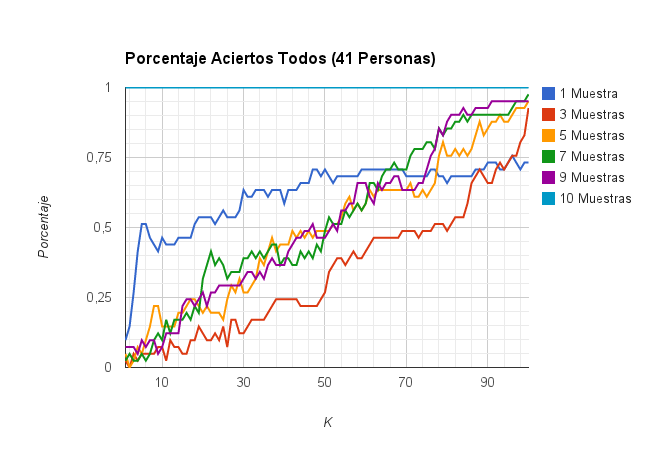
\includegraphics[width=1\textwidth]{img/imagel.png}
     \caption{Tiempos HitTodos \textcolor{red}{??} Matrix $A^tA$ con 41 personas variando K}
     \label{fig:figura1}
\end{figure}

\textbf{Mediciones de HitsCentro}

\begin{figure}[H]
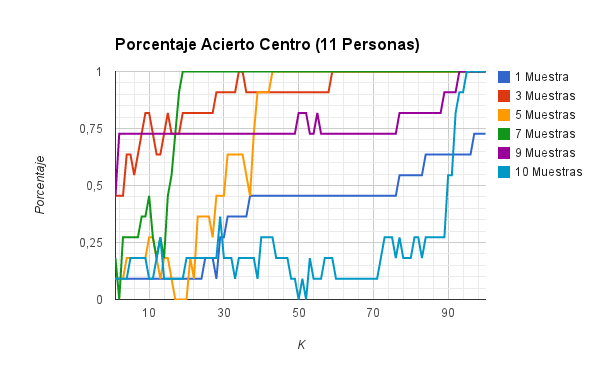
\includegraphics[width=1\textwidth]{img/imagem.png}
     \caption{Tiempos HitsCentro \textcolor{red}{??} Matrix $A^tA$ con 11 personas variando K}
     \label{fig:figura1}
\end{figure}

\begin{figure}[H]
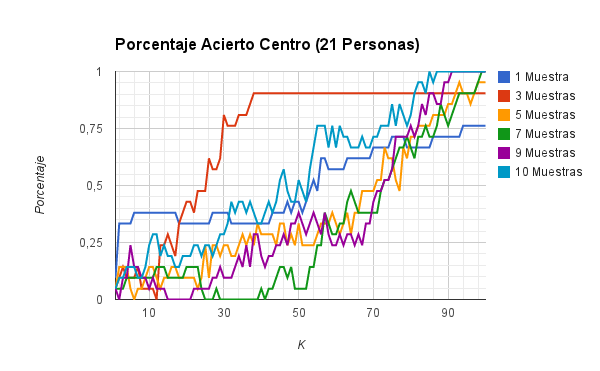
\includegraphics[width=1\textwidth]{img/imagen.png}
     \caption{Tiempos HitsCentro \textcolor{red}{??} Matrix $A^tA$ con 21 personas variando K}
     \label{fig:figura1}
\end{figure}

\begin{figure}[H]
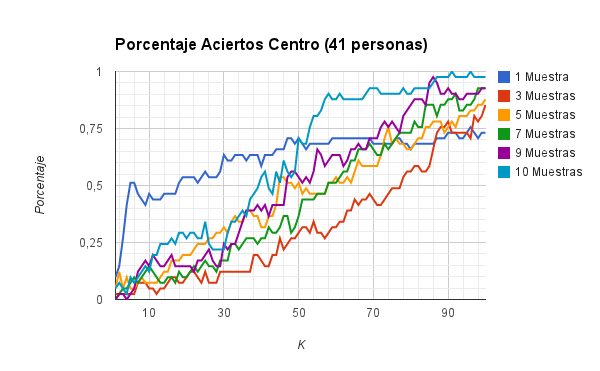
\includegraphics[width=1\textwidth]{img/imager.png}
     \caption{Tiempos HitsCentro \textcolor{red}{??} Matrix $A^tA$ con 41 personas variando K}
     \label{fig:figura1}
\end{figure}

\textbf{Conclusiones:}

\textcolor{red}{EXPLICAR}

\subsection{Experimentacion con Imagenes Full}

\subsubsection{Metodo 0: Utilizando $A^tA$}

\textbf{Mediciones de TK}

\textbf{Mediciones de Ttodos }

\textbf{Mediciones de Tcentro }

\textbf{Mediciones de HitsTodos }

\textbf{Mediciones de HitsCentro}

\textbf{Conclusiones:}

\textcolor{red}{EXPLICAR}

\subsubsection{Metodo 1: Utilizando $AA^t$}

\textbf{Mediciones de TK}

\begin{figure}[H]
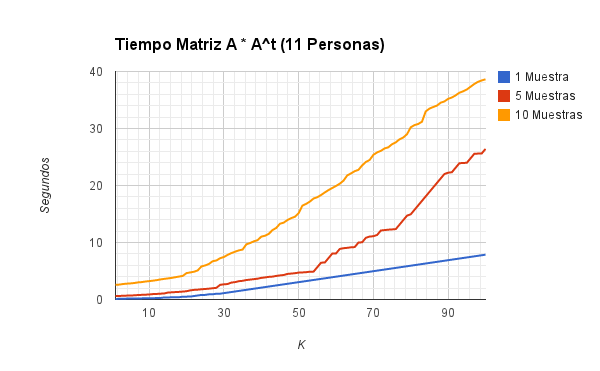
\includegraphics[width=1\textwidth]{img/imagef1.png}
     \caption{Tiempos HitsCentro \textcolor{red}{??} Matrix $A^tA$ con 41 personas variando K}
     \label{fig:figura1}
\end{figure}

\begin{figure}[H]
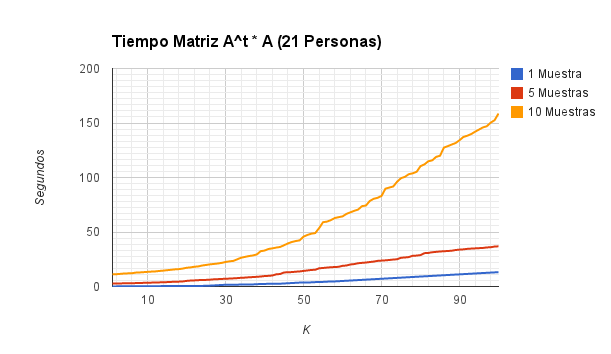
\includegraphics[width=1\textwidth]{img/imagef2.png}
     \caption{Tiempos HitsCentro \textcolor{red}{??} Matrix $A^tA$ con 41 personas variando K}
     \label{fig:figura1}
\end{figure}

\begin{figure}[H]
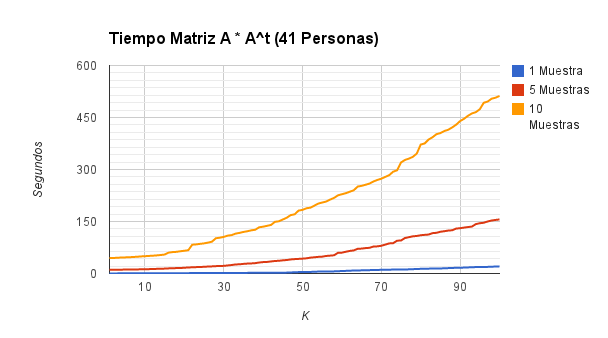
\includegraphics[width=1\textwidth]{img/imagef3.png}
     \caption{Tiempos HitsCentro \textcolor{red}{??} Matrix $A^tA$ con 41 personas variando K}
     \label{fig:figura1}
\end{figure}



\textbf{Mediciones de Ttodos }

\begin{figure}[H]
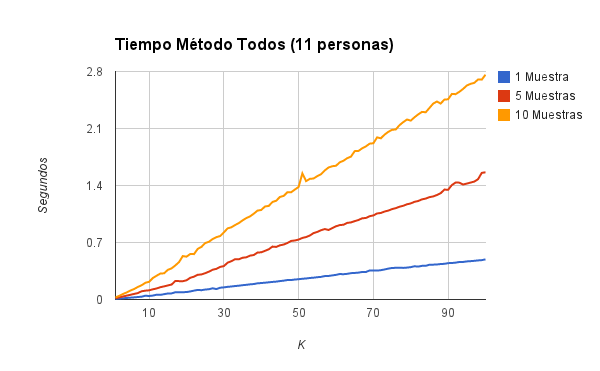
\includegraphics[width=1\textwidth]{img/imagef4.png}
     \caption{Tiempos HitsCentro \textcolor{red}{??} Matrix $A^tA$ con 41 personas variando K}
     \label{fig:figura1}
\end{figure}

\begin{figure}[H]
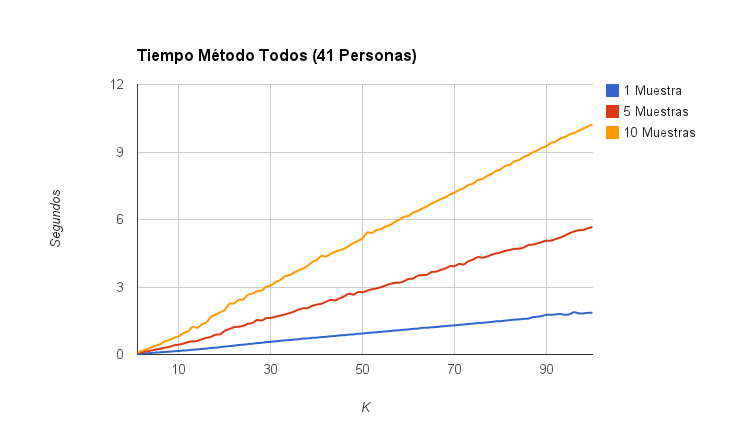
\includegraphics[width=1\textwidth]{img/imagef5.png}
     \caption{Tiempos HitsCentro \textcolor{red}{??} Matrix $A^tA$ con 41 personas variando K}
     \label{fig:figura1}
\end{figure}

\begin{figure}[H]
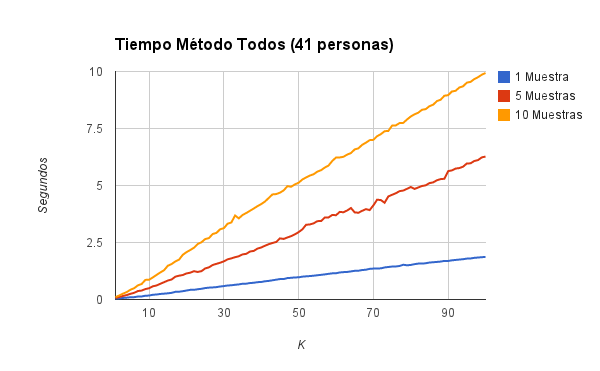
\includegraphics[width=1\textwidth]{img/imagef6.png}
     \caption{Tiempos HitsCentro \textcolor{red}{??} Matrix $A^tA$ con 41 personas variando K}
     \label{fig:figura1}
\end{figure}


\textbf{Mediciones de Tcentro }

\begin{figure}[H]
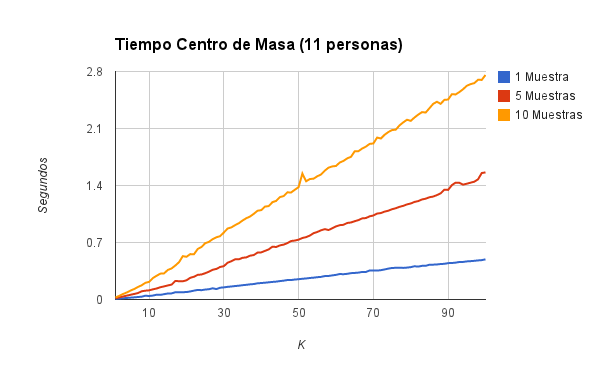
\includegraphics[width=1\textwidth]{img/imagef7.png}
     \caption{Tiempos HitsCentro \textcolor{red}{??} Matrix $A^tA$ con 41 personas variando K}
     \label{fig:figura1}
\end{figure}

\begin{figure}[H]
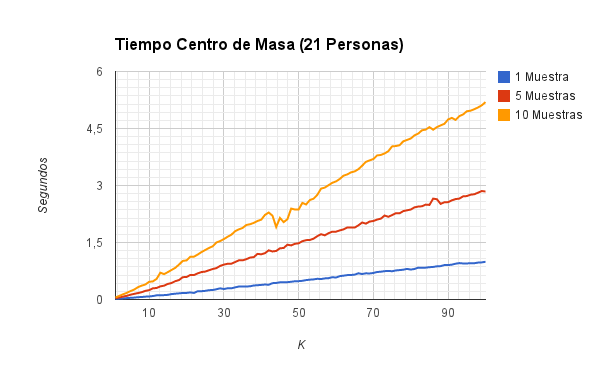
\includegraphics[width=1\textwidth]{img/imagef8.png}
     \caption{Tiempos HitsCentro \textcolor{red}{??} Matrix $A^tA$ con 41 personas variando K}
     \label{fig:figura1}
\end{figure}

\begin{figure}[H]
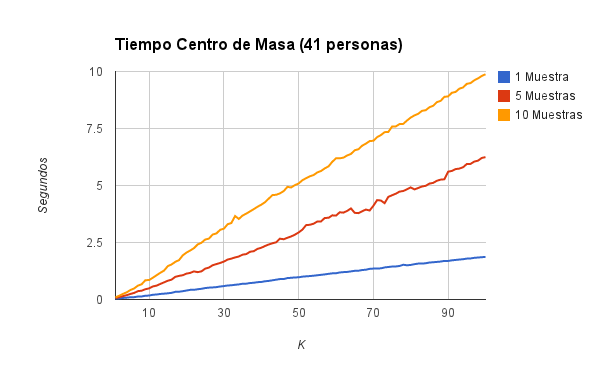
\includegraphics[width=1\textwidth]{img/imagef9.png}
     \caption{Tiempos HitsCentro \textcolor{red}{??} Matrix $A^tA$ con 41 personas variando K}
     \label{fig:figura1}
\end{figure}


\textbf{Mediciones de HitsTodos. }

\begin{figure}[H]
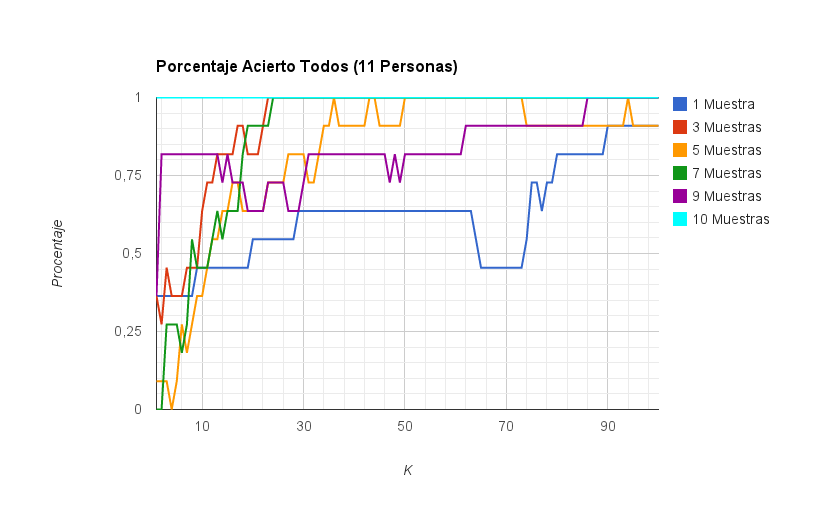
\includegraphics[width=1\textwidth]{img/imagef10.png}
     \caption{Tiempos HitsCentro \textcolor{red}{??} Matrix $A^tA$ con 41 personas variando K}
     \label{fig:figura1}
\end{figure}

\begin{figure}[H]
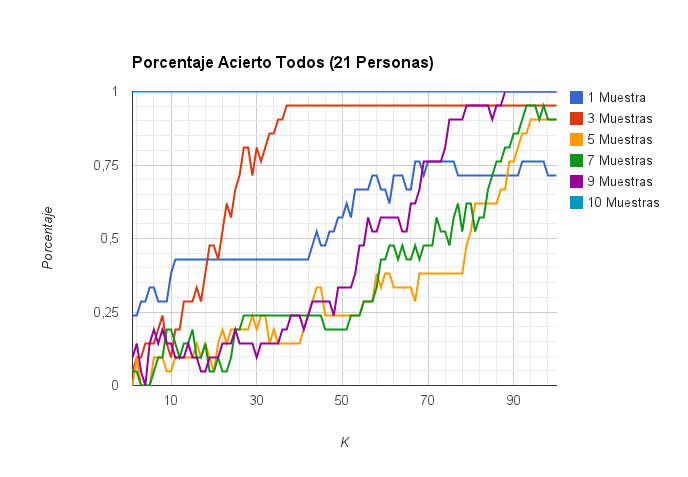
\includegraphics[width=1\textwidth]{img/imagef11.png}
     \caption{Tiempos HitsCentro \textcolor{red}{??} Matrix $A^tA$ con 41 personas variando K}
     \label{fig:figura1}
\end{figure}

\begin{figure}[H]
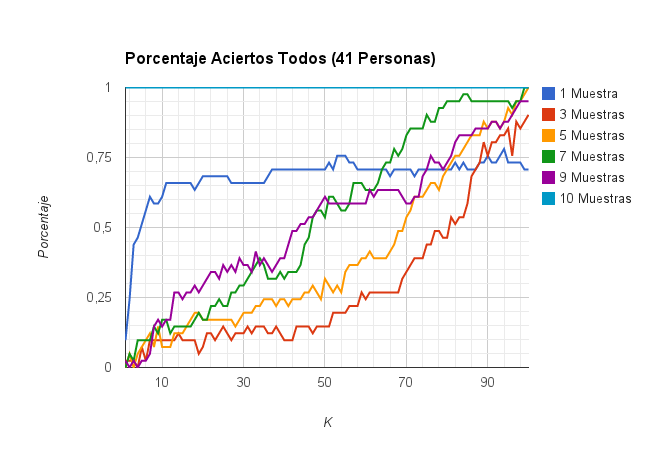
\includegraphics[width=1\textwidth]{img/imagef12.png}
     \caption{Tiempos HitsCentro \textcolor{red}{??} Matrix $A^tA$ con 41 personas variando K}
     \label{fig:figura1}
\end{figure}

\textbf{Mediciones de HitsCentro }

\begin{figure}[H]
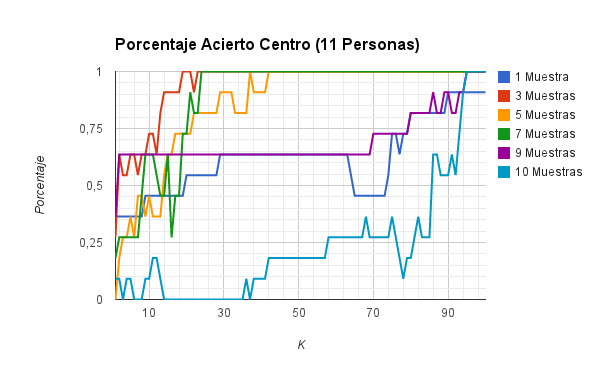
\includegraphics[width=1\textwidth]{img/imagef13.png}
     \caption{Tiempos HitsCentro \textcolor{red}{??} Matrix $A^tA$ con 41 personas variando K}
     \label{fig:figura1}
\end{figure}

\begin{figure}[H]
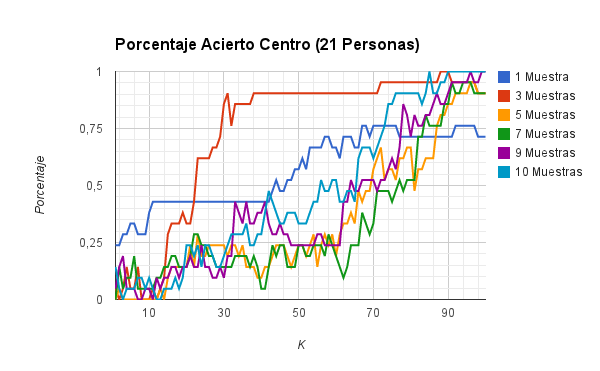
\includegraphics[width=1\textwidth]{img/imagef14.png}
     \caption{Tiempos HitsCentro \textcolor{red}{??} Matrix $A^tA$ con 41 personas variando K}
     \label{fig:figura1}
\end{figure}

\begin{figure}[H]
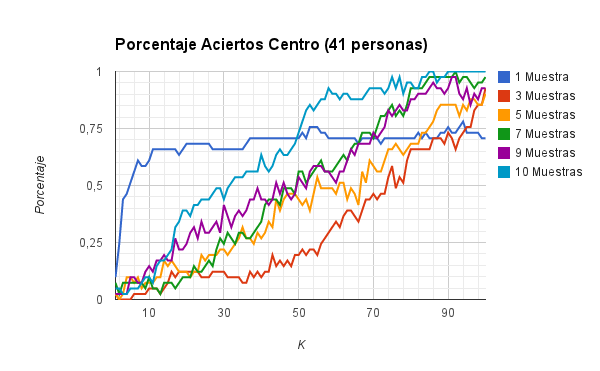
\includegraphics[width=1\textwidth]{img/imagef15.png}
     \caption{Tiempos HitsCentro \textcolor{red}{??} Matrix $A^tA$ con 41 personas variando K}
     \label{fig:figura1}
\end{figure}


\textbf{Conclusiones:}

\textcolor{red}{EXPLICAR}
